\documentclass{ieeeaccess}
\usepackage{cite}
\usepackage{amsmath,amssymb,amsfonts}
\usepackage{algorithm}
\usepackage{algorithmic}
\usepackage{graphicx}
\usepackage{textcomp}
\usepackage{booktabs}
\usepackage{url}

\usepackage{bm}
\makeatletter
\AtBeginDocument{\DeclareMathVersion{bold}
\SetSymbolFont{operators}{bold}{T1}{times}{b}{n}
\SetSymbolFont{NewLetters}{bold}{T1}{times}{b}{it}
\SetMathAlphabet{\mathrm}{bold}{T1}{times}{b}{n}
\SetMathAlphabet{\mathit}{bold}{T1}{times}{b}{it}
\SetMathAlphabet{\mathbf}{bold}{T1}{times}{b}{n}
\SetMathAlphabet{\mathtt}{bold}{OT1}{pcr}{b}{n}
\SetSymbolFont{symbols}{bold}{OMS}{cmsy}{b}{n}
\renewcommand\boldmath{\@nomath\boldmath\mathversion{bold}}}
\makeatother

\def\BibTeX{{\rm B\kern-.05em{\sc i\kern-.025em b}\kern-.08em
    T\kern-.1667em\lower.7ex\hbox{E}\kern-.125emX}}

% ---- short-hands used throughout
\newcommand{\Mz}{M_{0}}
\newcommand{\Mp}{M_{p}}
\newcommand{\caps}{\mathcal{C}}
\newcommand{\pools}{\mathcal{P}}
\newcommand{\own}{\pi}
\newcommand{\tvec}{\mathbf{t}}
\newcommand{\RAH}{RAH}
\graphicspath{{figures/}}

\begin{document}
\history{Date of publication xxxx 00, 0000, date of current version xxxx 00, 0000.}
\doi{10.1109/ACCESS.2026.0000000}

\title{Recoverability-Aware Healing: Pilot-Guided Allocation of Data Mixture and Adaptation Scope for Depth-Pruned Small Language Models}

% TODO (authors): affiliations, e-mails and the ORCID of the submitting author.
\author{\uppercase{Piyush Dhoka}\authorrefmark{1},
\uppercase{Vedant Pandhare}\authorrefmark{2},
\uppercase{Varun Inamdar}\authorrefmark{3},
\uppercase{Aadarsh Pathre}\authorrefmark{4},
\uppercase{Pavitha Nooji}\authorrefmark{5},
AND \uppercase{Sixth Author}\authorrefmark{6}}

\address[1]{Department, Institution, City, India (e-mail: author1@domain)}
\address[2]{Department, Institution, City, India (e-mail: author2@domain)}
\address[3]{Department, Institution, City, India (e-mail: author3@domain)}
\address[4]{Department, Institution, City, India (e-mail: author4@domain)}
\address[5]{Department, Institution, City, India (e-mail: author5@domain)}
\address[6]{Department, Institution, City, Country (e-mail: author6@domain)}
\tfootnote{This paragraph of the first footnote will contain support information (TODO: funding statement, or ``This work received no external funding.'').}

\markboth
{Dhoka \headeretal: Recoverability-Aware Healing of Depth-Pruned Small Language Models}
{Dhoka \headeretal: Recoverability-Aware Healing of Depth-Pruned Small Language Models}

\corresp{Corresponding author: Piyush Dhoka (e-mail: author1@domain).}

\begin{abstract}
Depth pruning, the removal of whole Transformer blocks, is a simple way to shrink small instruction-tuned language models for edge deployment, but it damages capabilities unevenly, and the short fine-tuning run that follows, called healing, has a fixed token budget. Current practice spreads that budget uniformly over a generic mixture or in proportion to how damaged each capability is. We argue that the budget should instead follow how recoverable each capability is. Recoverability-aware healing fits, from a few cheap pilot runs, a recovery curve for every capability together with a transfer matrix that captures how data for one capability helps another, then solves a concave program that jointly chooses the data mixture and the adaptation scope inside a trust region that forbids extrapolation. We evaluate six capabilities (structured output, function calling, instruction following, mathematical reasoning, safety refusal, and knowledge) on four model families with one to two billion parameters pruned by Block Influence, with three seeds and paired bootstrap tests. The order in which capabilities break is highly consistent across families, but damage does not predict recovery speed. At an equal budget, the proposed allocation is never worse than uniform healing on mean retention, raises the worst-retained capability by up to seventeen points, lowers over-refusal on three families without changing the balanced safety score, and beats damage-proportional allocation on two families while matching it on the other two. A pilot-free proxy did not work and is reported as a negative result. Code and all results are released.
\end{abstract}

\begin{keywords}
Depth pruning, function calling, instruction-tuned language models, layer pruning, low-rank adaptation, model compression, parameter-efficient fine-tuning, small language models, structured pruning.
\end{keywords}

\titlepgskip=-21pt

\maketitle

% =====================================================================
\section{Introduction}
\label{sec:introduction}
\PARstart{S}{mall} instruction-tuned language models with one to two billion parameters are what actually ships on phones, laptops, and low-cost cloud instances, increasingly as \emph{agents} that must emit schema-valid JSON, call tools with the right arguments, follow formatting instructions, and refuse unsafe requests. Every parameter of such a model costs memory, bandwidth, and energy, so compression matters. Depth pruning, which deletes entire Transformer blocks, is the simplest compression method with hardware-agnostic savings: each removed block cuts parameters, key--value cache, and per-token compute proportionally, without special kernels \cite{men2024shortgpt,gromov2024unreasonable,kim2024shortened,song2024sleb,muralidharan2024minitron}.

Depth pruning does not damage capabilities evenly. In our measurements, removing only two of the sixteen blocks of Llama-3.2-1B-Instruct leaves function calling at 0\% of its original score and structured output at 6\%, while safety refusal is untouched (Table~\ref{tab:damage}). The standard remedy is \emph{healing}: a short fine-tuning run on a modest amount of data \cite{gromov2024unreasonable,kim2024shortened,thangarasa2024selfdata}. Healing has a budget, measured in training tokens, and the budget has to be split across data that targets different capabilities. Common practice spreads it uniformly over a generic instruction mixture. The most recent allocation method, PASER \cite{he2026paser}, splits the recovery data across capability clusters \emph{in proportion to how much each capability has degraded}.

This article starts from a different premise: \emph{how damaged a capability is does not determine how recoverable it is}. Our pilot measurements show both kinds of mismatch. Structured output on Llama-3.2-1B is damaged by 91\% yet returns fully after about forty thousand tokens of healing data; mathematical reasoning on SmolLM2-1.7B is damaged by 91\% and barely moves no matter how many tokens it receives. A damage-proportional rule spends the same share of the budget on both. We therefore propose \emph{Recoverability-Aware Healing} (\RAH). Instead of inferring recoverability from damage, \RAH{} measures it: 21 small pilot heals, one healing pool at a time, are scored on every capability; a saturating recovery curve (a ceiling and a time-scale) is fitted per capability together with a non-negative transfer matrix that records how data for one capability helps another; and a small concave program then chooses the data mixture and the adaptation scope that maximize predicted retention at the full budget. The pilot-and-fit strategy itself comes from recent data-mixing optimizers for supervised fine-tuning \cite{li2025datamixing,domainpilot2026}; what is new is its use for healing, where the fitted quantities are recoverability ceilings and speeds relative to the unpruned model rather than losses, the adaptation scope is part of the decision, and three safeguards keep the optimizer inside what the pilots can support: a lower bound on the fitted time-scale, a trust region on tokens per pool, and an objective capped at the unpruned model's score. The pilots cost 3.5 times the tokens of one heal, a price we account for explicitly.

We evaluate the method on four open model families (Llama-3.2-1B, Qwen2.5-1.5B, SmolLM2-1.7B, and OLMo-2-1B) pruned with Block Influence \cite{men2024shortgpt}, on six capabilities that matter for deployed agents, with three seeds for every core method and item-level paired bootstrap tests. The contributions are as follows.
\begin{itemize}
\item A capability-level diagnosis of depth pruning in sub-2B instruction-tuned models covering structured output (JSONSchemaBench), function calling (BFCL), instruction following (IFEval), mathematical reasoning (GSM8K), safety and over-refusal (XSTest), and knowledge with calibration (MMLU, ECE). The breakage order is highly consistent across the four families (Kendall's $W = 0.92$): function calling and math break first, safety and knowledge last.
\item \RAH, which carries pilot-fitted mixture optimization \cite{li2025datamixing} over to post-pruning recovery: a recovery model fitted from 21 pilot runs that cost 3.5 times the tokens of one full heal, and a concave allocation of data mixture and adaptation scope with explicit safeguards against extrapolation. A capped variant of the objective was pre-registered before the last family's results were available.
\item Evidence that damage does not predict recovery \emph{speed} on any family and predicts recovery \emph{ceilings} on only two of four, so that an allocation rule that reads damage alone is working from incomplete information.
\item A controlled comparison at an equal budget of one million tokens. \RAH{} is never worse than uniform healing on the pre-registered primary metric and significantly better on two families; it raises the worst-retained capability by $+0.17$ (Llama) and $+0.14$ (OLMo); it beats damage-proportional allocation on Llama (worst case) and Qwen (mean) and ties on SmolLM2 and OLMo. Scope selection from pilots avoids losses of 0.05--0.18 in mean retention on three of four families.
\item Variants reported plainly: a max--min objective raises the worst-retained capability but pushes mean retention below uniform healing; a pilot-free proxy calibrated across families and a training-free linear patch fail to beat uniform healing; and a compute-matched comparison shows that a longer uniform heal can match \RAH{} once the pilot tokens are counted.
\item A reproducible pipeline that runs on an 8\,GB laptop GPU, released with teacher-data recipes, per-item predictions, and all results.
\end{itemize}

Section~\ref{sec:related} reviews related work. Section~\ref{sec:setting} fixes notation and the problem. Section~\ref{sec:method} presents \RAH. Section~\ref{sec:setup} describes the experimental setup, Section~\ref{sec:results} the results, Section~\ref{sec:discussion} the discussion and limitations, and Section~\ref{sec:conclusion} concludes.

% =====================================================================
\section{Related Work}
\label{sec:related}

\subsection{Depth Pruning of Language Models}
ShortGPT \cite{men2024shortgpt} scores each block by its Block Influence, one minus the cosine similarity between the block's input and output hidden states, and removes the lowest-scoring blocks. Gromov \emph{et al.} \cite{gromov2024unreasonable} remove a contiguous span chosen by angular distance and heal with QLoRA \cite{dettmers2023qlora} on generic text. Shortened LLaMA \cite{kim2024shortened} compares retraining recipes after depth pruning; SLEB \cite{song2024sleb} and LLM-Streamline \cite{chen2024streamline} refine the selection or replace removed spans with light modules; Minitron \cite{muralidharan2024minitron,sreenivas2024minitronpractice} combines depth and width pruning with distillation. Reassessing Layer Pruning \cite{lu2024reassessing} reports that tuning only the last layers after pruning beats LoRA, and CLP \cite{clp2025} tunes the blocks at the cut endpoints. Layer pruning with a consensus criterion has also appeared in this journal for convolutional networks \cite{mugnaini2025consensus}. Other granularities, such as unstructured sparsity \cite{frantar2023sparsegpt,sun2024wanda} and structured width pruning \cite{ma2023llmpruner,xia2024sheared}, are orthogonal to the question studied here. All of the depth-pruning work above fixes a single healing recipe and reports aggregate perplexity or multiple-choice accuracy; none allocates the healing budget across capabilities or chooses the adaptation scope.

\subsection{Repairs at the Cut}
Training-free or lightly trained patches align hidden states across a removed span: LinearPatch \cite{linearpatch2025}, Ghosted Layers \cite{ghosted2026}, and RestoreLCC \cite{restorelcc2025}. We include a ridge-regression linear patch in this spirit as a training-free baseline; it is far behind every trained method at our scale.

\subsection{Healing Data and Recovery Recipes}
PASER \cite{he2026paser} clusters the recovery instructions by capability and allocates the data budget across clusters in proportion to their measured degradation, for width and unstructured pruning of 7B-and-larger models evaluated on perplexity and multiple-choice tasks. It is the closest method to ours and the direct foil: \RAH{} replaces damage by measured recoverability, adds the adaptation scope to the decision, and targets depth-pruned sub-2B models on generative and agentic capabilities. Self-Data Distillation \cite{thangarasa2024selfdata} regenerates the healing targets with the unpruned model, which we adopt as the shared recipe for all methods; ShortOPD \cite{shortopd2026} distills on-policy. Closest in mechanism, although not in setting, are data-mixing optimizers for supervised fine-tuning. Li \emph{et al.} \cite{li2025datamixing} parametrize each domain's validation loss by the effective data transferred from every other domain under a fine-tuning scaling law, fit the parameters from small-scale mixture runs, and solve for the mixture weights; DomainPilot \cite{domainpilot2026} is a concurrent two-stage variant that fits per-domain convergence curves and then cross-domain interactions from sweeps. \RAH{} applies the same pilot-and-fit idea to healing, with three differences that the setting forces: the fitted quantities are recoverability ceilings and time-scales relative to the unpruned model, measured on task scores rather than loss, because loss and capability diverge after pruning \cite{jaiswal2024truth}; the adaptation scope is part of the decision; and the time-scale bound, trust region, and capped objective guard against the noisy pilots that a pruned model and a 60-item development set produce. Sheared-LLaMA's dynamic batch loading \cite{xia2024sheared} and DoReMi \cite{xie2023doremi} reweight pretraining domains online from loss gaps; they are precedents for adaptive mixtures but operate at pretraining scale and at the domain level. RankAdaptor \cite{rankadaptor2024} allocates LoRA rank per layer of a pruned model with a learned performance model; \RAH{} allocates data and scope instead, with a model fitted from direct pilot measurements. The free-lunch view of post-pruning retraining \cite{freelunch2025} and task-specific pruning studies \cite{taskpruning2026} examine how much fine-tuning recovers without asking how to split the budget.

\subsection{What Breaks Under Compression}
Shrestha \emph{et al.} \cite{limits2026layer} show that generative reasoning (math, code) is the most fragile capability under layer pruning and recovers least. A smart-home study \cite{smarthome2026} finds that tool-calling specificity breaks before intent and that false refusals rise sharply after pruning. LLM-KICK \cite{jaiswal2024truth} shows that compressed models can look intact on perplexity while failing knowledge-intensive tasks; width pruning of Llama-3.2 can even improve instruction following \cite{llama32pruning2025}. Quantization has similar uneven effects on safety and reliability \cite{kharinaev2026quantsafety}, and compression shifts refusal behavior itself \cite{xu2024beyondperplexity,chhabra2025refusal}. These studies diagnose but do not allocate. Finally, Alahmari \emph{et al.} \cite{alahmari2024repeatability} document in this journal that QLoRA fine-tuning runs are not repeatable across seeds, which is why every core method here is run with three seeds and compared with paired item-level tests.

% =====================================================================
\section{Problem Setting}
\label{sec:setting}

\subsection{Depth Pruning}
A decoder-only Transformer \cite{vaswani2017attention} $\Mz$ with $L$ blocks maps the residual stream $\mathbf{h}_{l-1}$ to $\mathbf{h}_{l}$ through block $l$. Block Influence \cite{men2024shortgpt} measures how much a block changes its input,
\begin{equation}
\mathrm{BI}_l = 1 - \mathbb{E}_{x,t}\!\left[\frac{\mathbf{h}_{l-1,t}^{\top}\mathbf{h}_{l,t}}{\lVert\mathbf{h}_{l-1,t}\rVert\,\lVert\mathbf{h}_{l,t}\rVert}\right],
\label{eq:bi}
\end{equation}
averaged over calibration tokens $t$ (the first position, which acts as an attention sink, is excluded; block~0 is never removed). The pruned model $\Mp$ removes the $k$ blocks with the lowest $\mathrm{BI}_l$; the kept blocks are re-indexed so that key--value caching stays correct.

\subsection{Capabilities, Pools, and Retention}
We track a set $\caps$ of six capabilities, written fmt, tool, inst, math, safe, and know (structured output, function calling, instruction following, mathematical reasoning, safety refusal, and knowledge). Healing data comes from a set $\pools$ of six pools, one per generative capability plus a general pool (fmt, tool, inst, math, safe, and general), with an own-pool map $\own(c)$ that is the identity except $\own(\text{know}) = \text{general}$. The retention of capability $c$ by a model $M$ is
\begin{equation}
r_c(M) = \frac{\mathrm{score}_c(M)}{\mathrm{score}_c(\Mz)},
\label{eq:retention}
\end{equation}
and its damage is $d_c = 1 - r_c(\Mp)$. Retention can exceed~1 when healing data teaches a format that the unpruned model handled poorly; exceeding the unpruned model is not recovery, so the pre-registered primary metrics are the \emph{capped mean retention} and the \emph{worst-case retention},
\begin{align}
\bar r^{\,\mathrm{cap}}(M) &= \frac{1}{|\caps|}\sum_{c\in\caps}\min\{r_c(M),1\}, \label{eq:metrics}\\
r^{\min}(M) &= \min_{c\in\caps} r_c(M). \label{eq:worst}
\end{align}
The uncapped mean, over-refusal, and calibration error are secondary.

\subsection{The Healing-Allocation Problem}
A healing run is specified by a token vector $\tvec = (t_p)_{p\in\pools}$ with $\sum_p t_p = B$ and by an adaptation scope $\sigma \in \Sigma = \{\text{all-LoRA},\text{cut-LoRA},\text{last-}k\}$, where all-LoRA places low-rank adapters \cite{hu2022lora} on every block, cut-LoRA only on the kept blocks that border a removed span \cite{clp2025}, and last-$k$ fully fine-tunes the last $k$ blocks and the final normalization \cite{lu2024reassessing}. Everything else (pools, teacher targets, optimizer, schedule, sequence length) is shared. The problem is to choose $(\tvec,\sigma)$ before the full heal so that the healed model's retention is as high as possible. Two rules from the literature serve as baselines:
\begin{align}
\text{uniform:}\quad & t_p = B/|\pools|, \label{eq:uniform}\\
\text{damage-proportional:}\quad & t_p \propto \sum_{c:\,\own(c)=p}\max\{0,\,d_c\}, \label{eq:dprop}
\end{align}
the second being the allocation rule of PASER \cite{he2026paser} applied to our pools (its within-cluster sample selection is not applicable to teacher-regenerated pools of equal quality).

% =====================================================================
\section{Recoverability-Aware Healing}
\label{sec:method}
Fig.~\ref{fig:overview} summarizes the pipeline. \RAH{} inserts three cheap steps between diagnosis and the full heal: pilot heals, a fitted recovery model, and an allocation solve.

\begin{figure*}[t]
\centering
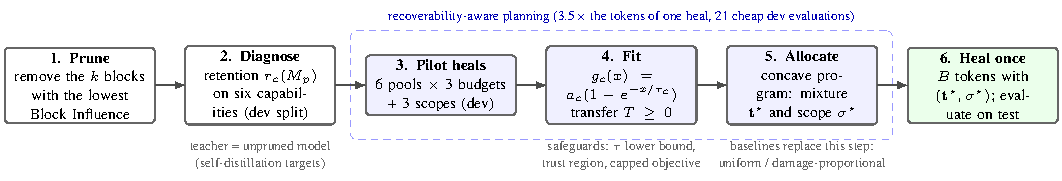
\includegraphics[width=\textwidth]{fig1_overview.pdf}
\caption{Pipeline. After pruning and diagnosis on the development split, \RAH{} runs 21 small pilot heals, fits a recovery curve per capability and a transfer matrix, and solves a concave program for the data mixture and the adaptation scope. The baselines replace only the allocation step; the full heal and the test evaluation are identical for every method.}
\label{fig:overview}
\end{figure*}

\subsection{Recovery Model}
The gain in retention of capability $c$ after healing with $x$ \emph{effective} tokens is modeled as a saturating exponential,
\begin{equation}
g_c(x) = a_c\left(1 - e^{-x/\tau_c}\right),\qquad a_c \ge 0,\ \tau_c > 0,
\label{eq:curve}
\end{equation}
where $a_c$ is the \emph{recovery ceiling}, the most retention this recipe can give back, and $\tau_c$ is the \emph{time-scale}, the number of tokens that recovers 63\% of the ceiling. A hyperbolic alternative $g_c(x) = a_c x/(x+\tau_c)$ is tested as an ablation. Data from one pool can help another capability (instruction data improves JSON validity, any instruction data improves multiple-choice knowledge), so the effective tokens of capability $c$ are a non-negative linear combination of pool tokens,
\begin{equation}
x_c(\tvec) = \sum_{p\in\pools} T_{cp}\,t_p,\qquad T_{c,\own(c)} = 1,\quad T_{cp}\ge 0.
\label{eq:effective}
\end{equation}
Normalizing the own-pool coefficient to~1 removes the scale ambiguity between $T$ and $\tau_c$; the non-negativity constraint keeps the allocation problem concave (negative interference is visible in the raw pilot table and is reported descriptively). The predicted retention after healing is
\begin{equation}
\hat r_c(\tvec) = \min\{r_c(\Mp) + g_c(x_c(\tvec)),\ r_{\max}\},\qquad r_{\max} = 1.2 .
\label{eq:predict}
\end{equation}

\subsection{Pilot Design}
For each pool $p\in\pools$ and each budget $b\in\{30\mathrm{k},100\mathrm{k},300\mathrm{k}\}$ tokens, $\Mp$ is healed with pool $p$ alone under the all-LoRA scope and evaluated on \emph{every} capability using the development split (60 items per capability), giving $6\times 3 = 18$ recovery pilots in which the own-pool points identify $(a_c,\tau_c)$ and the cross-pool points identify the row $T_{c,\cdot}$. Three further scope pilots heal $\Mp$ with the uniform mixture at 300k tokens under each scope in $\Sigma$. Two budget points per pool can fit a ceiling and a time-scale exactly and leave no slack for noise: a two-point design in a preliminary run produced a fit that assigned 97\% of the budget to one pool on the strength of an extrapolated curve; the third point is what makes the fit checkable. The development and test splits are disjoint, so the test split never informs any choice made by \RAH.

\subsection{Fitting}
For each capability $c$ the unknowns are $a_c$, $\tau_c$, and the five off-diagonal entries of $T_{c,\cdot}$, fitted to the 18 observed gains $\Delta r_c(p,b) = r_c(\text{pilot}_{p,b}) - r_c(\Mp)$ by bounded, ridge-regularized nonlinear least squares,
\begin{equation}
\min_{a_c,\tau_c,T_{c,\cdot}}\ \sum_{p,b}\Big(\Delta r_c(p,b) - g_c(T_{cp}\,b)\Big)^2 + \lambda\!\!\sum_{p\ne\own(c)}\! T_{cp}^2,
\label{eq:fit}
\end{equation}
with $\lambda = 0.05$, $0 \le a_c \le r_{\max} - r_c(\Mp)$, $T_{cp}\in[0,3]$, and $\tau_c \in [0.1\,b_{\min},\ 200\,b_{\max}]$. The lower bound on $\tau_c$ matters: a recovery faster than anything the pilots can resolve is not identifiable, and an unbounded $\tau_c \to 0$ makes the optimizer treat that capability as saturated at zero tokens. The ridge term shrinks transfer toward zero unless the pilots clearly show it. The fit is solved with a trust-region reflective least-squares routine; the residual root-mean-square error is reported per capability (Table~\ref{tab:fit}).

\subsection{Allocation}
With weights $w_c$ (uniform in this article) the utilitarian objective is
\begin{equation}
\max_{\tvec\ge 0}\ \sum_{c\in\caps} w_c\,\hat r_c(\tvec)\quad\text{s.t.}\quad \sum_{p}t_p = B,\ \ t_p \le t_{\max}.
\label{eq:rahsum}
\end{equation}
Each $g_c$ is concave and non-decreasing, $x_c$ is affine in $\tvec$ with non-negative coefficients, and the minimum of a concave function and a constant is concave, so \eqref{eq:rahsum} is a concave maximization over a capped simplex. At an interior optimum the marginal value $\sum_c w_c T_{cp}\, g_c'(x_c)$ is equal across all pools that receive tokens, so the optimum depends on ceilings and time-scales jointly, and a rule that reads damage alone cannot reproduce it in general. The problem is solved with sequential least-squares programming from 15 starts (uniform, six one-pool-concentrated, eight Dirichlet) in milliseconds. The \emph{trust region} $t_{\max} = 2\,b_{\max} = 600\mathrm{k}$ tokens stops the optimizer from relying on the curve far beyond the budgets at which it was measured; it is relaxed to $B/|\pools|$ when $B > |\pools|\,t_{\max}$. A max--min variant maximizes $\min_c \hat r_c(\tvec)$ in epigraph form; it is also concave.

\textbf{Capped objective.} Because the primary metric caps retention at~1, predicted retention above~1 should earn nothing. \RAH-capped replaces $\hat r_c$ in \eqref{eq:rahsum} by $\min\{\hat r_c,1\}$. This variant was pre-registered after the Llama and SmolLM2 main results and before the OLMo results were available, when it became clear that the uncapped objective was spending 54--60\% of the budget on capabilities predicted to exceed the unpruned model.

\subsection{Scope Selection}
The scope pilots give, for each scope $\sigma$, the development retention $r_c(\sigma)$ of every capability after a 300k-token uniform heal. \RAH{} picks $\sigma^\star = \arg\max_\sigma \sum_c w_c\, r_c(\sigma)$ (for the max--min variant, $\arg\max_\sigma \min_c r_c(\sigma)$). The baselines use all-LoRA, the scope of the recovery pilots. Per-capability winners are reported as well, since they differ.

\subsection{Pilot-Free Proxy}
To test whether the pilots can be skipped, \RAH-proxy estimates the ceilings from the increase in the negative log-likelihood of the teacher's own responses after pruning, $\Delta\mathrm{NLL}_c = \mathrm{NLL}_{\Mp} - \mathrm{NLL}_{\Mz}$ on 50 examples of pool $\own(c)$, a Monte-Carlo estimate of the divergence between teacher and pruned model on that capability. A linear map $\hat a_c = \alpha + \beta\,\Delta\mathrm{NLL}_c$ is calibrated on \emph{another} family's fitted ceilings, the time-scale is that family's median $\tau$, and $T = I$. The cross-family calibration is what keeps the proxy honest; it never sees its own family's pilots.

\subsection{Full Heal and Cost}
Algorithm~\ref{alg:rah} lists the procedure. The pilots process $6\times(30+100+300)\mathrm{k} + 3\times 300\mathrm{k} = 3.48\mathrm{M}$ tokens, 3.5 times one full heal at $B = 1\mathrm{M}$, plus 21 development evaluations of 60 items per capability. Once fitted, the recovery model can be re-solved for any budget or priority weights in milliseconds, so the pilot cost is amortized over every deployment that shares the pruned model. Section~\ref{sec:compute} compares this cost against spending the same tokens on a longer heal.

\begin{algorithm}[t]
\caption{Recoverability-Aware Healing}
\label{alg:rah}
\begin{algorithmic}[1]
\REQUIRE pruned model $\Mp$, teacher pools $\{D_p\}$, budget $B$, pilot budgets $\{b\}$, scopes $\Sigma$
\STATE evaluate $r_c(\Mp)$ on the development split for all $c\in\caps$
\FOR{each pool $p\in\pools$ and budget $b$}
  \STATE heal $\Mp$ with $b$ tokens of $D_p$ (all-LoRA); record $\Delta r_c(p,b)$ for all $c$
\ENDFOR
\FOR{each scope $\sigma\in\Sigma$}
  \STATE heal $\Mp$ with the uniform mixture at $300\mathrm{k}$ tokens under $\sigma$; record $r_c(\sigma)$
\ENDFOR
\STATE fit $(a_c,\tau_c,T_{c,\cdot})$ for every $c$ by \eqref{eq:fit}
\STATE $\tvec^\star \leftarrow$ solve \eqref{eq:rahsum} with the trust region (capped variant: $\min\{\hat r_c,1\}$)
\STATE $\sigma^\star \leftarrow \arg\max_\sigma \sum_c w_c\,r_c(\sigma)$
\STATE heal $\Mp$ once with $(\tvec^\star,\sigma^\star)$ at budget $B$; evaluate on the test split
\end{algorithmic}
\end{algorithm}

% =====================================================================
\section{Experimental Setup}
\label{sec:setup}

\subsection{Models and Pruning}
Table~\ref{tab:models} lists the four families \cite{grattafiori2024llama3,qwen2025qwen25,allal2025smollm2,olmo2025olmo2}. Block Influence is computed on a stream of 126 teacher examples (21 per pool), cut into 256-token chunks, with a beginning-of-sequence token prepended where the tokenizer defines one and the first position excluded from the average. The number of removed blocks was set per family so that capabilities are damaged but not all at chance: removing four of Llama-3.2-1B's sixteen blocks (25\%) left five of six capabilities at their chance floor (structured output 0.00, function calling 0.00, math 0.005, safety 0.51, knowledge 0.21), which makes damage uninformative, so Llama and OLMo-2-1B (same depth) remove two blocks, Qwen2.5-1.5B removes seven of 28, and SmolLM2-1.7B four of 24. A lighter cut is evaluated for diagnosis only. Llama is loaded from an ungated public mirror of the official checkpoint; the other three are the official repositories.

\begin{table*}[t]
\caption{Model families, Block-Influence cuts (original block indices; block~0 is never removed), and the hardware each family ran on.}
\label{tab:models}
\centering\footnotesize
\resizebox{\textwidth}{!}{\begin{tabular}{llrrllll}
\toprule
Family & Checkpoint & Params & Blocks & Removed (main) & Removed (light) & Hardware \\
\midrule
Llama-3.2-1B & unsloth/Llama-3.2-1B-Instruct & 1.24B & 16 & 12, 13 (12.5\%) & 12 & RTX 4060 Laptop (8 GB); L4 for two seeds \\
Qwen2.5-1.5B & Qwen/Qwen2.5-1.5B-Instruct & 1.54B & 28 & 13, 14, 15, 16, 24, 25, 26 (25.0\%) & 15, 16, 25, 26 & RTX 4060 Laptop (8 GB) \\
SmolLM2-1.7B & HuggingFaceTB/SmolLM2-1.7B-Instruct & 1.71B & 24 & 6, 20, 21, 22 (16.7\%) & 21, 22 & A100 (40 GB) \\
OLMo-2-1B & allenai/OLMo-2-0425-1B-Instruct & 1.48B & 16 & 8, 13 (12.5\%) & 13 & A100 (40 GB) \\
\bottomrule
\end{tabular}
}
\end{table*}

\subsection{Evaluation Suite}
Table~\ref{tab:evalsuite} summarizes the suite. Items are fixed, seeded subsets so that every checkpoint of a family sees identical inputs; the test split is used only for final numbers, the development split only for pilots. Generation is greedy with per-capability length caps and each model's own chat template. Structured output asks for a JSON object valid under a JSONSchemaBench schema \cite{geng2025jsonschemabench}; function calling presents BFCL v3 simple and multiple-function items \cite{patil2025bfcl} with the schemas in the system prompt and scores name and arguments by abstract-syntax-tree matching; instruction following uses IFEval's strict prompt-level checkers \cite{zhou2023ifeval} through lm-evaluation-harness \cite{gao2024lmeval}; math is GSM8K exact match on the final number \cite{cobbe2021gsm8k}; safety uses 100 unsafe and 100 benign XSTest prompts \cite{rottger2024xstest} with a string-match refusal classifier, scoring refusal of unsafe prompts and compliance with benign ones (the balanced score) and reporting the over-refusal rate separately; knowledge scores MMLU \cite{hendrycks2021mmlu} by the log-likelihood of the answer letters and reports the expected calibration error (ECE, 10 bins) \cite{guo2017calibration}. Because the prompt formats are model-agnostic, absolute scores are lower than leaderboard numbers; the comparisons are all relative and paired.

\begin{table*}[t]
\caption{Evaluation suite. Test items give the final numbers; development items are used by the pilots. Knowledge uses log-likelihood scoring and generates nothing.}
\label{tab:evalsuite}
\centering\footnotesize
\begin{tabular}{llllrrl}
\toprule
Key & Capability & Benchmark & Test & Dev & Max new tokens & Score \\
\midrule
fmt & Structured output & JSONSchemaBench (GitHub-easy) & 150 & 60 & 256 & schema-valid JSON \\
tool & Function calling & BFCL v3 simple + multiple & 200 & 60 & 128 & AST match (name + arguments) \\
inst & Instruction following & IFEval & 300 & 60 & 384 & strict prompt-level accuracy \\
math & Mathematical reasoning & GSM8K test & 200 & 60 & 256 & exact final answer \\
safe & Safety refusal & XSTest (100 unsafe + 100 benign) & 200 & 60 & 64 & refuse unsafe, comply benign \\
know & Knowledge & MMLU (all subjects) & 300 & 60 & -- & letter log-likelihood accuracy; ECE \\
\bottomrule
\end{tabular}

\end{table*}

\subsection{Healing Pools and Teacher Targets}
Each pool starts from about 1,300 prompts whose sources are disjoint from the evaluation sets (Table~\ref{tab:pools}): function-calling prompts and JSON-instance tasks are built from glaive-function-calling-v2 schemas \cite{glaive2023functioncalling}; instruction-following prompts attach one of ten verifiable constraints (lowercase, no commas, exactly three bullets, end with a phrase, and so on) to Alpaca-cleaned instructions \cite{yahma2023alpacacleaned,taori2023alpaca}; math uses the GSM8K training split; the safety pool mixes harmful prompts from PKU-SafeRLHF \cite{ji2024pkusaferlhf} with benign Alpaca look-alikes; the general pool is Alpaca-cleaned. Targets are generated greedily by the unpruned model of the same family (self-distillation \cite{thangarasa2024selfdata}) and quality-filtered so that only outputs that exhibit the skill are kept (schema-valid JSON, a known function with JSON arguments, a passing IFEval check, a correct final answer); up to 1,000 examples per pool are retained. Every method uses the same pools and targets.

\begin{table*}[t]
\caption{Healing pools and teacher-data yield per family: examples kept after quality control (and the fraction of prompts whose teacher output passed the check).}
\label{tab:pools}
\centering\footnotesize
\resizebox{\textwidth}{!}{\begin{tabular}{lllrrrr}
\toprule
Pool & Prompt source & Teacher QC & Llama-3.2-1B & Qwen2.5-1.5B & SmolLM2-1.7B & OLMo-2-1B \\
\midrule
fmt & JSON instances for glaive function schemas & schema-valid & 986 (78\%) & 1000 (100\%) & 1000 (98\%) & 1000 (100\%) \\
tool & glaive-function-calling-v2 & known function + JSON args & 1000 (98\%) & 1000 (100\%) & 1000 (99\%) & 895 (69\%) \\
inst & Alpaca-cleaned + verifiable constraint & IFEval checker passes & 831 (64\%) & 970 (75\%) & 1000 (80\%) & 1000 (78\%) \\
math & GSM8K train & final answer correct & 861 (66\%) & 912 (70\%) & 685 (53\%) & 1000 (82\%) \\
safe & PKU-SafeRLHF harmful + Alpaca benign & none & 1000 (100\%) & 1000 (100\%) & 1000 (100\%) & 1000 (100\%) \\
general & Alpaca-cleaned & none & 1000 (100\%) & 1000 (100\%) & 1000 (100\%) & 1000 (100\%) \\
\bottomrule
\end{tabular}
}
\end{table*}

\subsection{Training Recipe}
All heals share one recipe: LoRA rank 16, $\alpha = 32$, dropout 0.05 on the query, key, value, output, gate, up, and down projections \cite{hu2022lora,mangrulkar2022peft}; learning rate $2\times10^{-4}$ for LoRA and $2\times10^{-5}$ for the full-rank last-$k$ scope ($k = 3$ blocks plus the final normalization, trained in 32-bit precision); AdamW without weight decay, 5\% linear warm-up then cosine decay, 16 sequences of at most 512 tokens per update, loss on response tokens only, bfloat16 autocast, gradient checkpointing, and gradient clipping at~1. The mixture draws examples from each pool without replacement until the pool's token quota is met (cycling if a pool is exhausted), so the realized token count per pool is within one example of the plan; the total is one million tokens for every main run.

\subsection{Methods Compared}
Uniform \eqref{eq:uniform} and damage-proportional \eqref{eq:dprop} allocation with all-LoRA; \RAH{} (sum objective) and \RAH-capped with the pilot-chosen scope; \RAH-maxmin; \RAH-proxy; last-$k$ with the uniform mixture, the recipe of \cite{lu2024reassessing}; and a training-free linear patch that fits, on the unpruned model, a ridge-regularized linear map from the hidden state entering each removed span to the state leaving it (16k calibration tokens, $\lambda = 0.01\,\mathrm{tr}(X^{\top}X)/d$) and applies it after the preceding kept block, in the spirit of \cite{linearpatch2025,ghosted2026}. Ablations remove the transfer matrix ($T = I$), remove scope selection (all-LoRA), or use the hyperbolic curve. A budget sweep on Qwen2.5-1.5B compares \RAH{} and uniform healing at 0.25M and 4M tokens.

\subsection{Metrics, Seeds, and Statistics}
The primary metrics \eqref{eq:metrics} were fixed on 2026-10-05, before any \RAH{} test result existed; the uncapped mean, over-refusal, harmful-prompt refusal, and ECE are secondary. Uniform, damage-proportional, \RAH, and \RAH-capped are run with three seeds (0, 1, 2); the remaining methods with one seed; the linear patch is deterministic. Statistics are computed at the item level: per-item scores are averaged over seeds, items are resampled within each capability (2,000 paired bootstrap resamples), and the resampled capped mean and worst case give confidence intervals and two-sided $p$-values for the difference between two methods. Damage--recoverability relations use Spearman's rank correlation over the six capabilities, and the consistency of the breakage order across families uses Kendall's coefficient of concordance $W$.

\subsection{Hardware and Software}
Llama-3.2-1B and Qwen2.5-1.5B ran on two RTX 4060 Laptop GPUs (8\,GB) under Windows with the GPU memory capped at 92\% to prevent silent spilling into shared memory; SmolLM2-1.7B and OLMo-2-1B ran on an A100 (40\,GB); the second and third seeds of \RAH-capped on Llama ran on an L4 (24\,GB) with teacher data verified identical by checksum. All runs use bfloat16, transformers 4.56.2 \cite{wolf2020transformers}, PEFT 0.21.2, and lm-evaluation-harness 0.4.13.

% =====================================================================
\section{Results}
\label{sec:results}

\subsection{What Breaks}
\label{sec:breakage}
Table~\ref{tab:damage} and Fig.~\ref{fig:breakage} show retention after pruning on the test split. Function calling collapses on every family (retention 0.00--0.05) and math is next (0.00--0.07), while safety refusal (0.77--1.02) and knowledge (0.57--0.87) are largely preserved. Structured output and instruction following sit in between and vary most across families (0.04--0.49 and 0.20--0.66). The mean breakage ranks are 1.4 (function calling), 1.9 (math), 2.8 (structured output), 4.0 (instruction following), 5.3 (knowledge), and 5.8 (safety), and the four rankings agree with $W = 0.92$. The failures of the generative skills are largely structural: after the main cut, Llama produces parseable JSON for 10\% of structured-output prompts and 6\% of function-calling prompts (99\% and 93\% before pruning), and Qwen for 16\% and 0\%. The lighter cut is not uniformly gentler: removing four of Qwen's 28 blocks already removes function calling and math entirely, whereas Llama keeps 75--90\% of everything but math at one removed block. Pruning also moves the safety operating point: Llama's over-refusal rises from 0.04 to 0.12 and OLMo's calibration error doubles (0.14 to 0.28).

\begin{table*}[t]
\caption{Retention after pruning on the test split, for the light and the main cut, with the absolute unpruned scores and the breakage ranks (1 = most damaged). $W$ is Kendall's coefficient of concordance of the four rankings.}
\label{tab:damage}
\centering\footnotesize
\begin{tabular}{llrrrrrr}
\toprule
Family & Quantity & Struct. & Tool & Instr. & Math & Safety & Knowl. \\
\midrule
Llama-3.2-1B & unpruned score & 0.32 & 0.54 & 0.45 & 0.47 & 0.62 & 0.32 \\
 & retention, light cut & 0.75 & 0.89 & 0.90 & 0.35 & 1.27 & 0.75 \\
 & retention, main cut & 0.06 & 0.00 & 0.43 & 0.07 & 1.02 & 0.76 \\
 & breakage rank (1 = worst) & 2 & 1 & 4 & 3 & 6 & 5 \\
\midrule
Qwen2.5-1.5B & unpruned score & 0.78 & 0.86 & 0.38 & 0.48 & 0.73 & 0.58 \\
 & retention, light cut & 0.11 & 0.00 & 0.28 & 0.01 & 0.88 & 0.65 \\
 & retention, main cut & 0.04 & 0.00 & 0.20 & 0.00 & 0.80 & 0.57 \\
 & breakage rank (1 = worst) & 3 & 1 & 4 & 1 & 6 & 5 \\
\midrule
SmolLM2-1.7B & unpruned score & 0.71 & 0.69 & 0.45 & 0.39 & 0.74 & 0.43 \\
 & retention, light cut & 0.52 & 0.38 & 0.60 & 0.12 & 0.96 & 0.86 \\
 & retention, main cut & 0.21 & 0.05 & 0.33 & 0.06 & 0.77 & 0.87 \\
 & breakage rank (1 = worst) & 3 & 1 & 4 & 2 & 5 & 6 \\
\midrule
OLMo-2-1B & unpruned score & 0.60 & 0.54 & 0.60 & 0.62 & 0.85 & 0.36 \\
 & retention, light cut & 0.76 & 0.87 & 0.86 & 0.06 & 0.91 & 0.99 \\
 & retention, main cut & 0.49 & 0.04 & 0.66 & 0.02 & 0.85 & 0.72 \\
 & breakage rank (1 = worst) & 3 & 2 & 4 & 1 & 6 & 5 \\
\midrule
All & mean rank ($W$ = 0.92) & 2.75 & 1.38 & 4.00 & 1.88 & 5.75 & 5.25 \\
\bottomrule
\end{tabular}

\end{table*}

\begin{figure}[t]
\centering
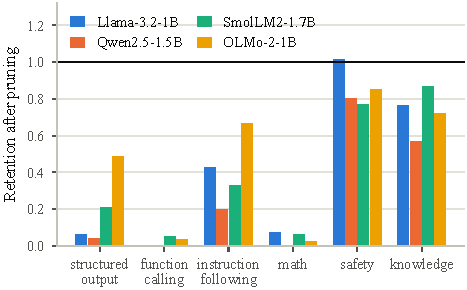
\includegraphics[width=\columnwidth]{fig2_breakage.pdf}
\caption{Retention after the main cut (test split). Function calling and math break first on every family; safety and knowledge are largely preserved.}
\label{fig:breakage}
\end{figure}

\subsection{Damage Does Not Determine Recoverability}
\label{sec:recoverability}
Table~\ref{tab:fit} and Figs.~\ref{fig:ceiling}--\ref{fig:transfer} report the fitted recovery models. Ceilings range from 0 to 1.13 and time-scales from the 3k lower bound of the fit (a recovery faster than the pilots can resolve) to 555k tokens, and the two are not tied to damage in any simple way. On Llama, structured output (damage 0.91) has a ceiling of 0.96 and a time-scale of 13k tokens, so it is fully recoverable with a few tens of thousands of tokens, whereas math (damage 0.93) has a ceiling above~1 but a time-scale of 530k tokens, forty times slower. On SmolLM2, math (damage 0.91) has a ceiling of 0.04: under this recipe it does not come back. On Qwen, safety is above the unpruned model already (ceiling 0) and knowledge gains at most 0.06. On OLMo, instruction following (damage 0.20) did not improve in any pilot (ceiling 0). The rank correlation between damage and ceiling is 0.77 (Llama), 0.67 (Qwen), $-0.09$ (SmolLM2), and 0.43 (OLMo), none significant with six capabilities; the correlation between damage and time-scale is 0.43, 0.03, $-0.14$, and $-0.77$. Damage is therefore a rough guide to \emph{how much} can come back on two families and no guide at all to \emph{how fast}, and the second quantity decides where a finite budget should go.

The transfer matrices (Fig.~\ref{fig:transfer}) are mostly small (below 0.3) with two systematic exceptions: knowledge benefits from every pool (for example, instruction and safety data count 0.64 and 0.68 of own-pool tokens on Llama, and instruction data 0.54 on OLMo), because any instruction data improves letter-choice answering on a pruned model; and on SmolLM2 function calling benefits from every pool (0.35--0.48). Negative interference exists in the raw pilot table (on Llama, 100k tokens of math data lowered function calling by 0.07) but is excluded from the fitted model by construction. The fit residuals (0.02--0.19 root-mean-square) reflect the 60-item development evaluations; the largest residuals occur for capabilities whose pilots fluctuate around~1.

\begin{table*}[t]
\caption{Fitted recovery models on the development split: damage, recovery ceiling $a_c$, time-scale $\tau_c$ (thousands of own-pool tokens; 3 is the lower bound of the fit and means faster than the pilots can resolve; n/a when the ceiling is zero), fit residual, and Spearman correlations between damage and the fitted quantities (six capabilities, none significant).}
\label{tab:fit}
\centering\footnotesize
\begin{tabular}{llrrrrrr}
\toprule
Family & Quantity & Struct. & Tool & Instr. & Math & Safety & Knowl. \\
\midrule
Llama-3.2-1B & damage $1-r_c$ & 0.91 & 1.00 & 0.59 & 0.93 & -0.08 & 0.48 \\
 & ceiling $a_c$ & 0.96 & 0.70 & 0.18 & 1.13 & 0.12 & 0.41 \\
 & time-scale $\tau_c$ (k tokens) & 13 & 35 & 3 & 530 & 3 & 52 \\
 & fit RMSE & 0.089 & 0.054 & 0.045 & 0.052 & 0.118 & 0.121 \\
 & $\rho$(damage, $a_c$) / $\rho$(damage, $\tau_c$) & \multicolumn{6}{c}{0.77 ($p$ = 0.07) / 0.43 ($p$ = 0.40)} \\
\midrule
Qwen2.5-1.5B & damage $1-r_c$ & 0.93 & 1.00 & 0.89 & 1.00 & -0.03 & 0.45 \\
 & ceiling $a_c$ & 0.67 & 0.37 & 0.33 & 0.10 & 0.00 & 0.06 \\
 & time-scale $\tau_c$ (k tokens) & 38 & 91 & 24 & 29 & n/a & 3 \\
 & fit RMSE & 0.052 & 0.016 & 0.107 & 0.028 & 0.189 & 0.066 \\
 & $\rho$(damage, $a_c$) / $\rho$(damage, $\tau_c$) & \multicolumn{6}{c}{0.67 ($p$ = 0.15) / 0.03 ($p$ = 0.96)} \\
\midrule
SmolLM2-1.7B & damage $1-r_c$ & 0.76 & 0.91 & 0.50 & 0.91 & 0.29 & 0.29 \\
 & ceiling $a_c$ & 0.58 & 0.66 & 0.70 & 0.04 & 0.39 & 0.27 \\
 & time-scale $\tau_c$ (k tokens) & 120 & 90 & 246 & 39 & 56 & 40 \\
 & fit RMSE & 0.100 & 0.079 & 0.110 & 0.066 & 0.075 & 0.058 \\
 & $\rho$(damage, $a_c$) / $\rho$(damage, $\tau_c$) & \multicolumn{6}{c}{-0.09 ($p$ = 0.87) / -0.14 ($p$ = 0.79)} \\
\midrule
OLMo-2-1B & damage $1-r_c$ & 0.29 & 0.97 & 0.20 & 0.94 & 0.08 & 0.50 \\
 & ceiling $a_c$ & 0.26 & 0.79 & 0.00 & 0.24 & 0.28 & 0.35 \\
 & time-scale $\tau_c$ (k tokens) & 37 & 15 & n/a & 136 & 555 & 29 \\
 & fit RMSE & 0.123 & 0.049 & 0.162 & 0.035 & 0.026 & 0.070 \\
 & $\rho$(damage, $a_c$) / $\rho$(damage, $\tau_c$) & \multicolumn{6}{c}{0.43 ($p$ = 0.40) / -0.77 ($p$ = 0.07)} \\
\bottomrule
\end{tabular}

\end{table*}

\begin{figure*}[t]
\centering
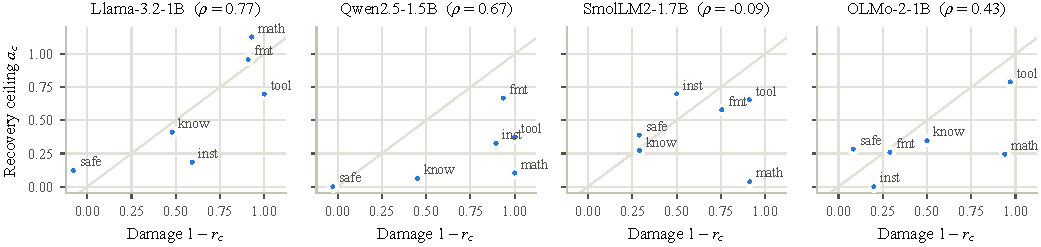
\includegraphics[width=\textwidth]{fig3_damage_vs_ceiling.pdf}
\caption{Damage versus fitted recovery ceiling per capability (development split). Points on the diagonal would be fully recoverable; points far below it are damaged but not recoverable under this recipe. $\rho$ is Spearman's correlation over the six capabilities.}
\label{fig:ceiling}
\end{figure*}

\begin{figure*}[t]
\centering
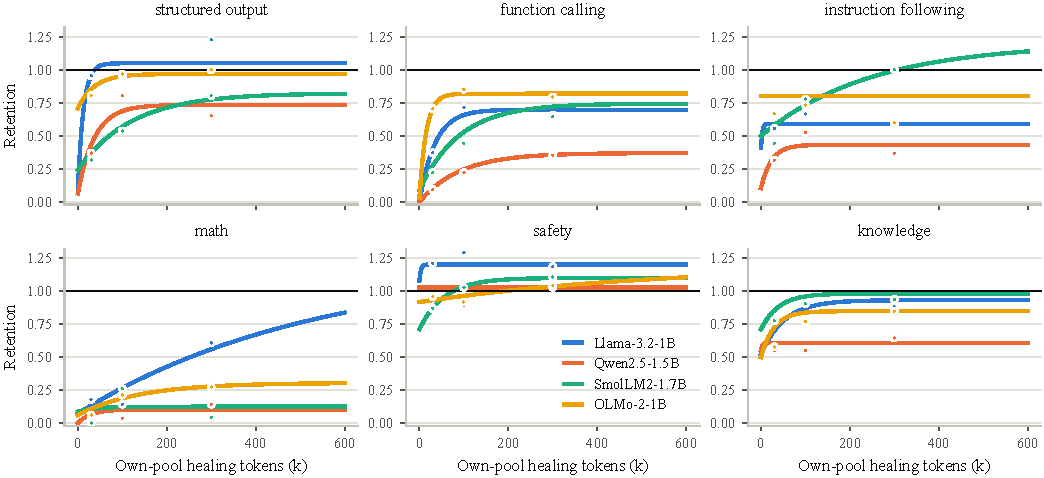
\includegraphics[width=\textwidth]{fig4_recovery_curves.pdf}
\caption{Fitted recovery curves \eqref{eq:curve} per capability with the own-pool pilot observations (dots) at 30k, 100k, and 300k tokens. The same capability recovers at very different speeds and to very different ceilings across families.}
\label{fig:curves}
\end{figure*}

\begin{figure*}[t]
\centering
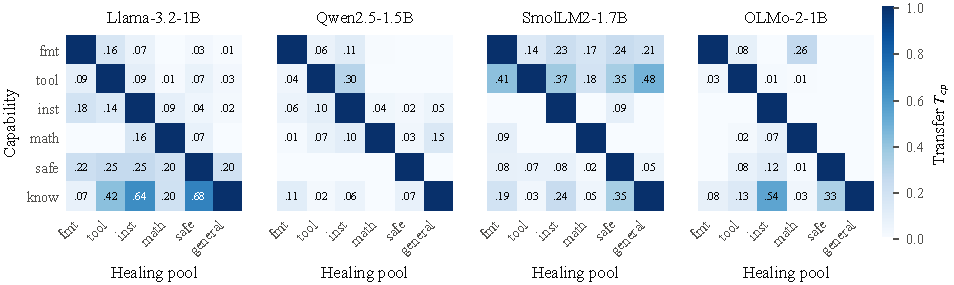
\includegraphics[width=\textwidth]{fig5_transfer.pdf}
\caption{Fitted transfer matrices $T_{cp}$: how many effective tokens one token of pool $p$ contributes to capability $c$ (own pool $= 1$). Knowledge benefits from every pool; most other transfer is small.}
\label{fig:transfer}
\end{figure*}

\subsection{The Allocations}
Fig.~\ref{fig:alloc} shows where each rule sends the budget. Damage-proportional allocation looks similar on every family because the damage profiles are similar (Section~\ref{sec:breakage}): roughly a quarter each to structured output, function calling, and math, and nothing to safety. \RAH{} differs sharply and family-specifically. On Llama it gives math the trust-region maximum (60\%), instruction following 20\%, function calling 15\%, and structured output only 4\%, since structured output saturates after a few tens of thousands of tokens; it also switches to the last-$k$ scope. On Qwen it gives function calling 52\% and structured output 24\%, and nothing to the safety and general pools whose capabilities have no headroom. On SmolLM2 and OLMo the uncapped objective exposed its failure mode: it sent 60\% to instruction following (SmolLM2) and 54\% to safety (OLMo) because those capabilities were predicted to exceed the unpruned model, which the capped metric does not reward; the capped objective moves the budget to structured output (52\%) on SmolLM2 and to math (60\%) on OLMo.

\begin{figure*}[t]
\centering
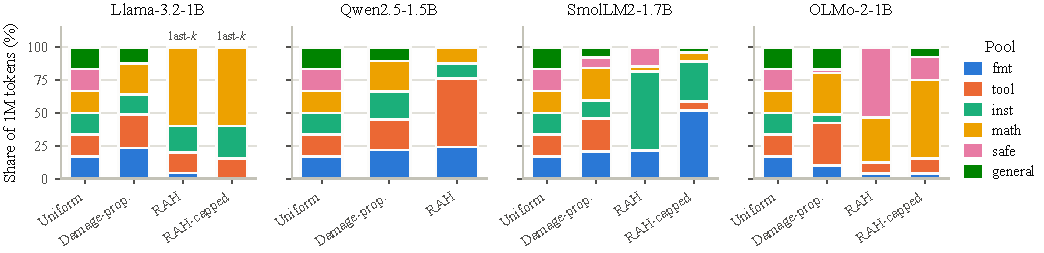
\includegraphics[width=\textwidth]{fig6_allocations.pdf}
\caption{Token allocation of the four methods at $B = 1$M (the scope is all-LoRA unless annotated). Damage-proportional allocation is nearly the same on every family; \RAH{} is family-specific. On Qwen, \RAH-capped coincides with \RAH{} because the only capability predicted above the unpruned model, safety, has a zero ceiling, so neither objective allocates to it.}
\label{fig:alloc}
\end{figure*}

\subsection{Main Comparison}
\label{sec:main}
Tables~\ref{tab:main} and \ref{tab:headline} and Figs.~\ref{fig:bymethod} and \ref{fig:headline} give the test results with three seeds per method.

\textbf{Llama-3.2-1B.} Capped mean retention is 0.82 (uniform), 0.83 (damage-proportional), 0.85 (\RAH), and 0.84 (\RAH-capped). \RAH{} beats uniform by $+0.031$ ($p = 0.014$) and damage-proportional by $+0.021$ ($p = 0.075$). The worst-retained capability, math, rises from 0.38 to 0.54 ($+0.17$ versus uniform, $p < 0.001$; $+0.12$ versus damage-proportional, $p = 0.02$), and instruction following from 0.67 to 0.76, at the cost of structured output (1.49 to 1.13 for the capped variant), which was already above the unpruned model. Damage-proportional allocation produces the highest \emph{uncapped} mean (1.07) by pushing structured output to twice its unpruned score; the capped metric discounts this, as intended.

\textbf{Qwen2.5-1.5B.} Capped mean retention is 0.62, 0.61, and 0.64; \RAH{} beats damage-proportional by $+0.024$ ($p = 0.039$) and uniform by $+0.020$ ($p = 0.145$). Worst-case retention is a tie, because math is essentially unrecoverable on this family (ceiling 0.10) under every mixture. The safety operating point differs strongly: the unpruned Qwen refuses 97\% of harmful and 51\% of benign XSTest prompts, the uniform mixture reproduces this behavior (100\% and 59\%), while \RAH, which assigns no tokens to the safety pool, refuses 50\% of harmful and 6\% of benign prompts; the balanced safety score is similar (0.96 versus 0.99 retention). \RAH-capped is identical to \RAH{} here.

\textbf{SmolLM2-1.7B.} All four methods tie on capped mean retention (0.76--0.78, $p > 0.29$ for every comparison). \RAH{} and \RAH-capped have a slightly lower worst case (0.10 versus 0.15; $p = 0.10$ and $p = 0.045$ against uniform and damage-proportional respectively) because they give math only 4--7\% of the budget on the strength of a 0.04 ceiling, whereas the baselines' 17--25\% math share still buys a little. \RAH-capped lowers over-refusal from 0.21 to 0.08, again by refusing less overall (harmful-prompt refusal 0.43 versus 0.75).

\textbf{OLMo-2-1B.} Damage-proportional allocation has the best capped mean (0.77): on this family the two most damaged capabilities, function calling and math, are also the two most recoverable, so the damage rule happens to coincide with recoverability, while the uncapped \RAH{} objective spent 54\% of the budget on safety (0.75). The capped objective repairs this: \RAH-capped reaches 0.76, better than uniform ($+0.025$, $p = 0.043$) and tied with damage-proportional ($-0.008$, $p = 0.44$), and has the best worst case, lifting math from 0.21 to 0.35 ($+0.14$ versus uniform, $p < 0.001$; $+0.04$ versus damage-proportional, $p = 0.11$).

Across the four families, \RAH{} (capped where it differs) is never worse than uniform healing on the primary metric and significantly better on two; against damage-proportional allocation it wins on two families and ties on two. On worst-case retention it gains $+0.17$ and $+0.14$ on Llama and OLMo, ties on Qwen, and loses 0.05 on SmolLM2. Seed-to-seed variation is substantial (structured-output retention on Llama varies by $\pm0.5$ between seeds of the same method), which is why the comparisons are paired at the item level and why single-seed numbers below are read with caution.

\begin{table*}[t]
\caption{Per-capability retention on the test split (three seeds; per-item scores averaged over seeds) and the headline metrics. Bold marks the best capped mean and worst case per family. Over-refusal is the fraction of benign XSTest prompts refused; ECE is the expected calibration error on MMLU.}
\label{tab:main}
\centering\scriptsize
\setlength{\tabcolsep}{3.5pt}
\begin{tabular}{llrrrrrrrrrrr}
\toprule
Family & Method & Struct. & Tool & Instr. & Math & Safety & Knowl. & Capped mean & Mean & Worst & Over-refusal & ECE \\
\midrule
Llama-3.2-1B & Uniform & 1.49 & 0.88 & 0.67 & 0.38 & 1.27 & 1.15 & 0.82 & 0.97 & 0.38 & 0.16 & 0.18 \\
 & Damage-prop. & 2.02 & 0.90 & 0.66 & 0.43 & 1.34 & 1.09 & 0.83 & 1.07 & 0.43 & 0.15 & 0.19 \\
 & RAH & 1.49 & 0.82 & 0.76 & 0.54 & 1.27 & 1.09 & \textbf{0.85} & 1.00 & 0.54 & 0.09 & 0.26 \\
 & RAH-capped & 1.13 & 0.77 & 0.74 & 0.55 & 1.28 & 1.11 & 0.84 & 0.93 & \textbf{0.55} & 0.09 & 0.27 \\
\midrule
Qwen2.5-1.5B & Uniform & 0.73 & 0.54 & 0.58 & 0.21 & 0.96 & 0.67 & 0.62 & 0.62 & \textbf{0.21} & 0.59 & 0.26 \\
 & Damage-prop. & 0.73 & 0.54 & 0.56 & 0.19 & 1.09 & 0.66 & 0.61 & 0.63 & 0.19 & 0.09 & 0.28 \\
 & RAH & 0.77 & 0.58 & 0.62 & 0.19 & 0.99 & 0.68 & \textbf{0.64} & 0.64 & 0.19 & 0.06 & 0.24 \\
 & RAH-capped & \multicolumn{11}{l}{identical allocation to RAH on this family (see Fig.~6)} \\
\midrule
SmolLM2-1.7B & Uniform & 0.90 & 0.93 & 0.70 & 0.15 & 1.04 & 0.96 & 0.77 & 0.78 & \textbf{0.15} & 0.21 & 0.20 \\
 & Damage-prop. & 0.87 & 0.92 & 0.68 & 0.14 & 1.04 & 0.96 & 0.76 & 0.77 & 0.14 & 0.19 & 0.21 \\
 & RAH & 0.88 & 0.96 & 0.78 & 0.10 & 1.06 & 0.91 & 0.77 & 0.78 & 0.10 & 0.19 & 0.26 \\
 & RAH-capped & 0.96 & 0.93 & 0.79 & 0.10 & 0.91 & 0.97 & \textbf{0.78} & 0.78 & 0.10 & 0.08 & 0.21 \\
\midrule
OLMo-2-1B & Uniform & 0.77 & 0.97 & 0.71 & 0.21 & 0.96 & 0.81 & 0.74 & 0.74 & 0.21 & 0.16 & 0.26 \\
 & Damage-prop. & 0.84 & 0.99 & 0.73 & 0.31 & 0.96 & 0.80 & \textbf{0.77} & 0.77 & 0.31 & 0.12 & 0.26 \\
 & RAH & 0.77 & 0.97 & 0.67 & 0.29 & 0.97 & 0.83 & 0.75 & 0.75 & 0.29 & 0.15 & 0.32 \\
 & RAH-capped & 0.78 & 0.98 & 0.66 & 0.35 & 0.98 & 0.83 & 0.76 & 0.76 & \textbf{0.35} & 0.16 & 0.23 \\
\bottomrule
\end{tabular}

\end{table*}

\begin{table*}[t]
\caption{Item-level paired bootstrap (2,000 resamples, seeds pooled) on the pre-registered metrics: differences, 95\% confidence intervals, and two-sided $p$-values.}
\label{tab:headline}
\centering\footnotesize
\begin{tabular}{llrrrr}
\toprule
Family & Comparison & $\Delta$ capped mean [95\% CI] & $p$ & $\Delta$ worst case [95\% CI] & $p$ \\
\midrule
Llama-3.2-1B & RAH vs Uniform & +0.031 [+0.006, +0.053] & 0.014 & +0.168 [+0.070, +0.267] & $<$0.001 \\
 & RAH vs Damage-prop. & +0.021 [-0.003, +0.045] & 0.075 & +0.116 [+0.021, +0.207] & 0.020 \\
 & RAH-capped vs Uniform & +0.021 [-0.006, +0.044] & 0.123 & +0.172 [+0.081, +0.270] & $<$0.001 \\
 & RAH-capped vs Damage-prop. & +0.011 [-0.016, +0.034] & 0.436 & +0.119 [+0.028, +0.211] & 0.012 \\
\midrule
Qwen2.5-1.5B & RAH vs Uniform & +0.020 [-0.007, +0.045] & 0.145 & -0.027 [-0.086, +0.031] & 0.369 \\
 & RAH vs Damage-prop. & +0.024 [+0.001, +0.042] & 0.039 & -0.007 [-0.069, +0.052] & 0.863 \\
\midrule
SmolLM2-1.7B & RAH vs Uniform & -0.001 [-0.023, +0.022] & 0.953 & -0.048 [-0.104, +0.009] & 0.101 \\
 & RAH vs Damage-prop. & +0.008 [-0.015, +0.036] & 0.453 & -0.043 [-0.095, +0.009] & 0.116 \\
 & RAH-capped vs Uniform & +0.003 [-0.021, +0.027] & 0.883 & -0.052 [-0.104, +0.004] & 0.076 \\
 & RAH-capped vs Damage-prop. & +0.013 [-0.012, +0.037] & 0.296 & -0.048 [-0.095, -0.004] & 0.045 \\
\midrule
OLMo-2-1B & RAH vs Uniform & +0.013 [-0.009, +0.034] & 0.251 & +0.075 [+0.027, +0.129] & 0.002 \\
 & RAH vs Damage-prop. & -0.020 [-0.039, +0.001] & 0.057 & -0.027 [-0.067, +0.011] & 0.176 \\
 & RAH-capped vs Uniform & +0.025 [+0.001, +0.048] & 0.043 & +0.142 [+0.083, +0.210] & $<$0.001 \\
 & RAH-capped vs Damage-prop. & -0.008 [-0.029, +0.012] & 0.436 & +0.040 [-0.008, +0.089] & 0.107 \\
\bottomrule
\end{tabular}

\end{table*}

\begin{figure*}[t]
\centering
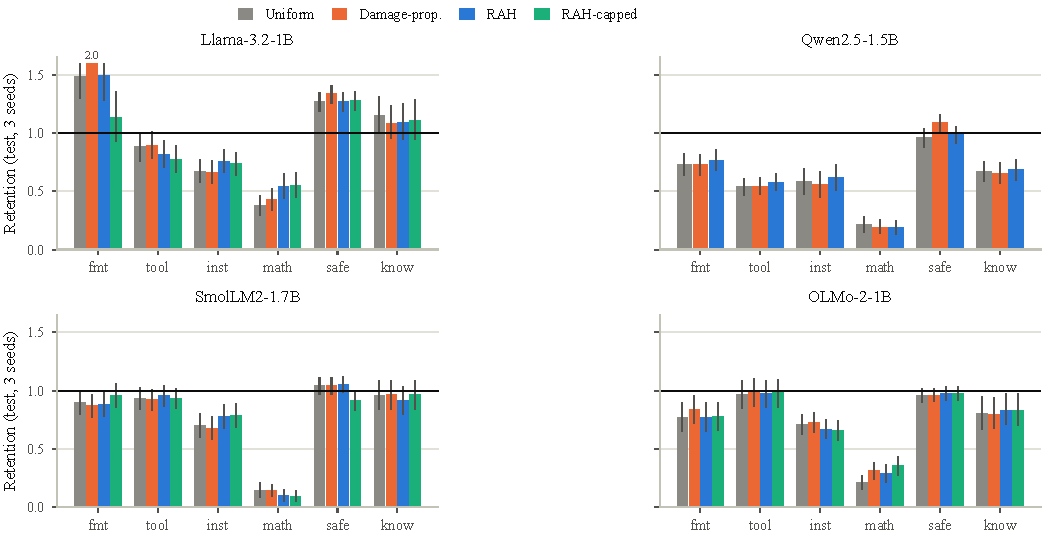
\includegraphics[width=\textwidth]{fig7_retention_by_method.pdf}
\caption{Retention by method and capability on the test split (three seeds; whiskers are 95\% bootstrap intervals over items). Values above~1 exceed the unpruned model; bars clipped at the axis top carry their value.}
\label{fig:bymethod}
\end{figure*}

\begin{figure*}[t]
\centering
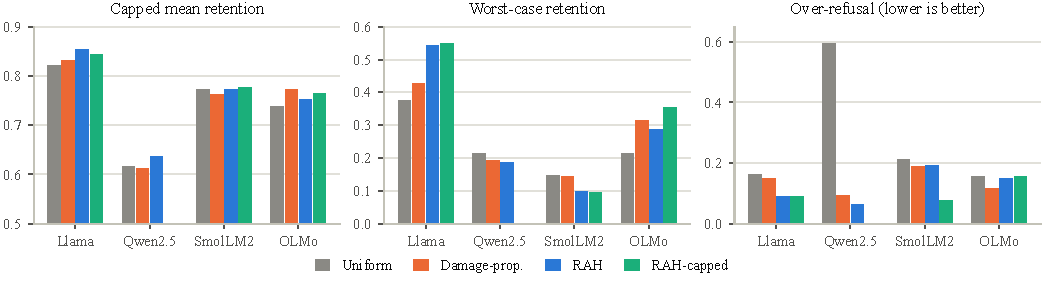
\includegraphics[width=\textwidth]{fig8_headline.pdf}
\caption{Headline metrics by family. \RAH{} is never below uniform healing on capped mean retention and raises the worst case strongly on Llama and OLMo; over-refusal moves with the share of the safety pool in the mixture.}
\label{fig:headline}
\end{figure*}

\subsection{Scope Matters, and Differs by Family}
Table~\ref{tab:scope} reports the scope pilots. Full fine-tuning of the last three blocks is the best scope on Llama (development capped mean 0.82 versus 0.78 for all-LoRA) and clearly the worst on the other three families (0.43, 0.47, and 0.64 versus 0.57, 0.68, and 0.72). The 1M-token main runs confirm the pilots: last-$k$ with the uniform mixture scores 0.83 versus 0.82 for all-LoRA on Llama, but 0.46 versus 0.62 on Qwen, 0.59 versus 0.77 on SmolLM2, and 0.69 versus 0.74 on OLMo, with worst-case retention of 0.06 on Qwen. The recipe of \cite{lu2024reassessing}, tuning only the last layers, therefore does not transfer across families at this scale, and a single 300k-token pilot per scope is enough to avoid losses of 0.16, 0.18, and 0.05 in mean retention on Qwen, SmolLM2, and OLMo. The best scope also differs by capability within a family: on Llama, instruction following, math, and safety recover best under last-$k$, structured output under cut-LoRA, and function calling and knowledge under all-LoRA; on OLMo, math prefers cut-LoRA and safety last-$k$. A per-capability scope cannot be realized in a single heal, so \RAH{} picks the scope that is best on the sum.

\begin{table*}[t]
\caption{Scope pilots (300k tokens, uniform mixture, development split) and the scope chosen by \RAH, with the 1M-token test check of last-$k$ against all-LoRA under the uniform mixture.}
\label{tab:scope}
\centering\footnotesize
\begin{tabular}{llrrrrrrrr}
\toprule
Family & Scope & Struct. & Tool & Instr. & Math & Safety & Knowl. & Capped mean & Worst \\
\midrule
Llama-3.2-1B & all-LoRA & 1.45 & 0.86 & 0.56 & 0.29 & 1.03 & 1.08 & 0.78 & 0.29 \\
 & cut-LoRA & 1.50 & 0.71 & 0.63 & 0.18 & 1.00 & 0.92 & 0.74 & 0.18 \\
 & last-$k$ (chosen) & 1.36 & 0.80 & 0.81 & 0.32 & 1.05 & 1.00 & 0.82 & 0.32 \\
 & 1M check: last-$k$ / all-LoRA, uniform mix & \multicolumn{8}{l}{capped mean 0.83 / 0.82, worst 0.49 / 0.38 (test split)} \\
\midrule
Qwen2.5-1.5B & all-LoRA (chosen) & 0.76 & 0.41 & 0.42 & 0.11 & 1.03 & 0.74 & 0.57 & 0.11 \\
 & cut-LoRA & 0.65 & 0.22 & 0.37 & 0.04 & 0.95 & 0.65 & 0.48 & 0.04 \\
 & last-$k$ & 0.46 & 0.11 & 0.42 & 0.07 & 0.95 & 0.58 & 0.43 & 0.07 \\
 & 1M check: last-$k$ / all-LoRA, uniform mix & \multicolumn{8}{l}{capped mean 0.46 / 0.62, worst 0.06 / 0.21 (test split)} \\
\midrule
SmolLM2-1.7B & all-LoRA (chosen) & 0.66 & 0.71 & 0.67 & 0.04 & 1.00 & 1.06 & 0.68 & 0.04 \\
 & cut-LoRA & 0.46 & 0.60 & 0.50 & 0.00 & 0.97 & 0.84 & 0.56 & 0.00 \\
 & last-$k$ & 0.39 & 0.36 & 0.28 & 0.04 & 1.08 & 0.74 & 0.47 & 0.04 \\
 & 1M check: last-$k$ / all-LoRA, uniform mix & \multicolumn{8}{l}{capped mean 0.59 / 0.77, worst 0.06 / 0.15 (test split)} \\
\midrule
OLMo-2-1B & all-LoRA (chosen) & 0.84 & 0.97 & 0.70 & 0.09 & 0.90 & 0.85 & 0.72 & 0.09 \\
 & cut-LoRA & 0.81 & 0.88 & 0.67 & 0.15 & 0.94 & 0.69 & 0.69 & 0.15 \\
 & last-$k$ & 0.81 & 0.68 & 0.70 & 0.03 & 0.98 & 0.65 & 0.64 & 0.03 \\
 & 1M check: last-$k$ / all-LoRA, uniform mix & \multicolumn{8}{l}{capped mean 0.69 / 0.74, worst 0.17 / 0.21 (test split)} \\
\bottomrule
\end{tabular}

\end{table*}

\subsection{Ablations, Variants, and Negative Results}
Table~\ref{tab:ablation} lists every variant (one seed each except \RAH). Removing the transfer matrix changes the mixtures substantially (on Llama, 25\% of the budget moves to the general pool) but changes the capped mean by at most 0.02, and on Qwen it is slightly better (0.65 versus 0.64) with a higher worst case. Removing scope selection costs 0.02 on Llama, the only family where \RAH{} chose a scope other than all-LoRA; on the other three families the ablation is the same configuration as \RAH's first seed (the OLMo run is bitwise identical), and its differences of at most 0.01 measure run-to-run nondeterminism. The hyperbolic curve gives 0.83, 0.63, 0.77, and 0.77: the curve family matters less than the measured ceilings and time-scales. The value of \RAH{} therefore lies mainly in the pilots themselves, with transfer and curve shape second-order.

The max--min objective does what it is designed to do and shows what it costs. It gives the least recoverable capability the trust-region maximum (60\% on math on every family) and raises the worst case above uniform healing on all four families (0.51, 0.27, 0.22, and 0.31 versus 0.38, 0.21, 0.15, and 0.21) and above \RAH{} on three, but the capped mean falls below uniform on three families (0.83, 0.60, 0.75, and 0.61 versus 0.82, 0.62, 0.77, and 0.74), and on OLMo its scope rule chose cut-LoRA, which lost function calling (0.17). With one seed these numbers are fragile, but the trade-off is the expected one: the sum objective with the cap is the better default unless the worst capability is all that matters. Two variants are negative results. The pilot-free proxy produces near-uniform allocations on every family, because the cross-family linear map turns the pruned-versus-teacher likelihood gap into nearly constant ceilings, and consequently scores within 0.015 of uniform healing everywhere, including Qwen's 0.63 over-refusal. The training-free linear patch reaches a capped mean of only 0.37--0.65 and a worst case of 0.07--0.13: a linear map at the cut restores some structure but no generative capability at this scale.

\begin{table*}[t]
\caption{Ablations, variants, and the training-free baseline (one seed each; \RAH{} with three seeds for reference). The mixture lists the percentage of the budget given to each pool.}
\label{tab:ablation}
\centering\footnotesize
\setlength{\tabcolsep}{4pt}
\begin{tabular}{lllcrrr}
\toprule
Family & Variant & Scope & Mixture \% (fmt/tool/inst/math/safe/general) & Capped mean & Worst & Over-refusal \\
\midrule
Llama-3.2-1B & RAH (3 seeds) & last-$k$ & 4 / 15 / 20 / 60 / 0 / 0 & 0.85 & 0.54 & 0.09 \\
 & RAH, no transfer & last-$k$ & 7 / 11 / 6 / 50 / 1 / 25 & 0.83 & 0.54 & 0.09 \\
 & RAH, no scope choice & all-LoRA & 4 / 15 / 20 / 60 / 0 / 0 & 0.83 & 0.52 & 0.19 \\
 & RAH, hyperbolic curve & last-$k$ & 13 / 27 / 0 / 60 / 0 / 0 & 0.83 & 0.56 & 0.12 \\
 & RAH-maxmin & last-$k$ & 8 / 8 / 8 / 60 / 8 / 8 & 0.83 & 0.51 & 0.17 \\
 & RAH-proxy & all-LoRA & 21 / 18 / 18 / 14 / 11 / 18 & 0.82 & 0.37 & 0.13 \\
 & Last-$k$ + uniform & last-$k$ & 17 / 17 / 17 / 17 / 17 / 17 & 0.83 & 0.49 & 0.16 \\
 & Linear patch & -- & -- & 0.65 & 0.13 & 0.04 \\
\midrule
Qwen2.5-1.5B & RAH (3 seeds) & all-LoRA & 24 / 52 / 11 / 12 / 0 / 0 & 0.64 & 0.19 & 0.06 \\
 & RAH, no transfer & all-LoRA & 14 / 24 / 9 / 53 / 0 / 0 & 0.65 & 0.27 & 0.06 \\
 & RAH, no scope choice & all-LoRA & 24 / 52 / 11 / 12 / 0 / 0 & 0.63 & 0.15 & 0.02 \\
 & RAH, hyperbolic curve & all-LoRA & 34 / 51 / 5 / 10 / 0 / 0 & 0.63 & 0.16 & 0.05 \\
 & RAH-maxmin & all-LoRA & 8 / 8 / 8 / 60 / 8 / 8 & 0.60 & 0.27 & 0.56 \\
 & RAH-proxy & all-LoRA & 17 / 17 / 17 / 17 / 17 / 17 & 0.63 & 0.25 & 0.63 \\
 & Last-$k$ + uniform & last-$k$ & 17 / 17 / 17 / 17 / 17 / 17 & 0.46 & 0.06 & 0.71 \\
 & Linear patch & -- & -- & 0.37 & 0.07 & 0.33 \\
\midrule
SmolLM2-1.7B & RAH (3 seeds) & all-LoRA & 21 / 0 / 60 / 4 / 15 / 0 & 0.77 & 0.10 & 0.19 \\
 & RAH, no transfer & all-LoRA & 29 / 20 / 29 / 0 / 12 / 9 & 0.77 & 0.08 & 0.18 \\
 & RAH, no scope choice & all-LoRA & 21 / 0 / 60 / 4 / 15 / 0 & 0.78 & 0.14 & 0.21 \\
 & RAH, hyperbolic curve & all-LoRA & 25 / 0 / 54 / 0 / 21 / 0 & 0.77 & 0.09 & 0.26 \\
 & RAH-maxmin & all-LoRA & 8 / 8 / 8 / 60 / 8 / 8 & 0.75 & 0.22 & 0.24 \\
 & RAH-proxy & all-LoRA & 17 / 17 / 17 / 17 / 16 / 16 & 0.76 & 0.13 & 0.23 \\
 & Last-$k$ + uniform & last-$k$ & 17 / 17 / 17 / 17 / 17 / 17 & 0.59 & 0.06 & 0.32 \\
 & Linear patch & -- & -- & 0.49 & 0.08 & 0.25 \\
\midrule
OLMo-2-1B & RAH (3 seeds) & all-LoRA & 4 / 8 / 0 / 34 / 54 / 0 & 0.75 & 0.29 & 0.15 \\
 & RAH, no transfer & all-LoRA & 17 / 8 / 0 / 25 / 27 / 23 & 0.75 & 0.30 & 0.16 \\
 & RAH, no scope choice & all-LoRA & 4 / 8 / 0 / 34 / 54 / 0 & 0.74 & 0.27 & 0.16 \\
 & RAH, hyperbolic curve & all-LoRA & 2 / 14 / 0 / 44 / 40 / 1 & 0.77 & 0.37 & 0.16 \\
 & RAH-maxmin & cut-LoRA & 0 / 0 / 40 / 60 / 0 / 0 & 0.61 & 0.31 & 0.03 \\
 & RAH-proxy & all-LoRA & 17 / 17 / 16 / 17 / 15 / 17 & 0.75 & 0.25 & 0.17 \\
 & Last-$k$ + uniform & last-$k$ & 17 / 17 / 17 / 17 / 17 / 17 & 0.69 & 0.17 & 0.11 \\
 & Linear patch & -- & -- & 0.61 & 0.09 & 0.06 \\
\bottomrule
\end{tabular}

\end{table*}

\subsection{Budget Sweep}
Fig.~\ref{fig:budget} shows the Qwen sweep. At 0.25M tokens \RAH{} is below uniform (0.52 versus 0.55 mean retention): the fitted mixture (38\% function calling, 35\% structured output, 21\% instruction following, 6\% math, nothing for the safety and general pools) loses more on the capabilities it starves than it gains on the ones it targets at this budget. At 1M it is above (0.64 versus 0.62, three seeds). At 4M the trust region ($600\mathrm{k}$ per pool, relaxed to $B/|\pools|$) forces the uniform allocation, so the two runs train on the same mixture with the same seed; their difference of 0.003 is a measurement of run-to-run nondeterminism rather than of the method. The sweep therefore says that the pilot-fitted allocation pays off at moderate budgets and must not be trusted far below the budgets at which the curves were measured. Read as a compute-matched comparison, the 4M uniform run also exceeds \RAH{} at 1M (capped mean 0.66 versus 0.64); Section~\ref{sec:compute} discusses this.

\begin{figure}[t]
\centering
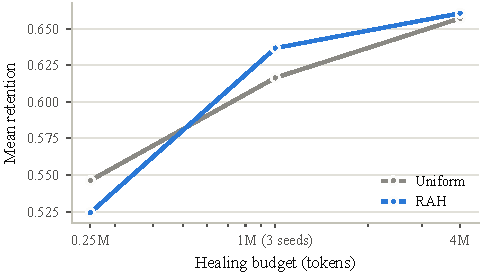
\includegraphics[width=\columnwidth]{fig9_budget_sweep.pdf}
\caption{Budget sweep on Qwen2.5-1.5B (mean retention; one seed at 0.25M and 4M, three seeds at 1M). At 4M the trust region makes the two allocations identical.}
\label{fig:budget}
\end{figure}

\subsection{Side Effects: Refusal and Calibration}
Over-refusal is governed by the share of the safety pool and by the teacher's own behavior. The unpruned Llama refuses 28\% of harmful and 4\% of benign prompts; every healed Llama refuses more of both (66--81\% and 9--16\%), and \RAH, which allocates nothing to the safety pool, refuses the least. The unpruned Qwen refuses 97\% of harmful and 51\% of benign prompts, so uniform healing, which includes the safety pool, faithfully restores an over-refusing teacher. The balanced XSTest score moves little across methods (0.91--1.09 retention); what the allocation changes is the operating point. Calibration moves in the other direction: healing lowers the ECE of pruned Llama from 0.48 to 0.17--0.19 under uniform and damage-proportional allocation but only to 0.26--0.27 under \RAH, whose last-$k$ full fine-tuning and math-heavy mixture increase confidence; on OLMo the uncapped \RAH{} has the highest ECE (0.32). A calibration term in the objective would be a natural extension.

% =====================================================================
\section{Discussion}
\label{sec:discussion}

\subsection{When Recoverability-Aware Allocation Helps}
\RAH{} helps when the recoverability profile departs from the damage profile: on Llama, where a cheap-to-restore capability (structured output) and an expensive one (math) are equally damaged, and on Qwen, where function calling has headroom and math has none. It ties when every mixture saturates the recoverable capabilities (SmolLM2) or when the damage rule coincidentally matches recoverability (OLMo, where it took the capped objective to match damage-proportional allocation). It also removes a hidden choice from the baselines: the uniform mixture's fixed share of safety data moved Qwen to a 59\% over-refusal operating point, whereas \RAH{} allocates safety data only where the pilots show headroom.

\subsection{What the Pilots Cost}
\label{sec:compute}
The comparisons of Section~\ref{sec:results} hold the healing budget fixed at 1M tokens for every method, which is the question a practitioner with a fixed budget asks. They do not hold total training compute fixed: \RAH's pilots process 3.48M tokens before the heal, so spending the same total on a longer uniform heal is a legitimate alternative. The one such comparison available cuts against \RAH: on Qwen2.5-1.5B, uniform healing with 4M tokens reaches a capped mean retention of 0.66 against 0.64 for \RAH{} at 1M (Fig.~\ref{fig:budget}). The pilots therefore pay for themselves in two situations: when the heal itself is budget-limited, by memory, time, or a token cap imposed by a deployment pipeline, and when the fitted recovery model is reused, since re-planning for a different budget or different priority weights is a millisecond solve and the pilots double as a diagnosis of which capabilities can come back at all. For a single heal with no token limit, a longer uniform heal may simply be the better use of the compute. A compute-matched sweep on all four families is the obvious next experiment; we did not run it.

\subsection{A Practitioner's Recipe}
Run the 21 pilots (3.5 times the tokens of one heal, each evaluated on 60 items per capability), fit the model with the $\tau$ lower bound and the ridge term, use the capped objective, keep the trust region, and choose the scope from the scope pilots. The fitted model is reusable: a new budget, new deployment weights $w_c$, or a different cap changes the solve, not the pilots. The decision to run pilots is the cost--benefit one of Section~\ref{sec:compute}: at this scale they gain 0.02--0.03 in capped mean and up to 0.17 in worst-case retention at a fixed budget, which is worth 3.5 heals when the pruned model will be deployed widely or re-healed for several budgets, and not worth it for a one-off model with a generous budget.

\subsection{Threats to Validity and Limitations}
\emph{Scale.} All families are between 1.2B and 1.7B parameters; whether the profiles persist at 3B--8B is untested. \emph{Evaluation size.} Test subsets of 150--300 items give confidence intervals of about $\pm0.1$ per capability, and development sets of 60 items make the pilots noisy (fit residuals up to 0.19). \emph{Single pruning criterion and recipe.} Block Influence and teacher-regenerated targets are held fixed; the ceilings are properties of this recipe, and a stronger healing recipe may raise them. \emph{Three budget points per pool.} Ceilings beyond 300k tokens are extrapolated; the trust region limits but does not remove this risk, and the 0.25M sweep shows the fitted allocation can mislead far below the pilot budgets. \emph{Refusal classifier.} A string-match classifier over-counts polite non-refusals and under-counts indirect ones; the over-refusal numbers should be read as operating points, not precise rates. \emph{Seeds.} Variants other than the four core methods use one seed. \emph{Hardware.} Two GPU types were used; the L4 seeds used checksum-identical data, and the 4M-token repeat quantifies run-to-run nondeterminism at 0.003 mean retention. \emph{Compute.} The baselines are matched on healing tokens, not on total compute (Section~\ref{sec:compute}). \emph{Language.} All data are English.

% =====================================================================
\section{Conclusion}
\label{sec:conclusion}
Depth pruning of sub-2B instruction-tuned models breaks function calling and math first and safety and knowledge last, consistently across four families, but how much and how fast each capability comes back is family-specific and only loosely related to how badly it broke. Recoverability-Aware Healing measures recoverability with cheap pilot heals and turns the measurement into an allocation of healing data and adaptation scope by a concave program with explicit safeguards. At an equal healing budget it is never worse than uniform healing on the pre-registered metric, improves the worst-retained capability by up to 0.17, and matches or beats damage-proportional allocation on every family; the scope choice alone avoids losses of up to 0.18 on three of four families. The pilots cost 3.5 times the tokens of one heal, and when that compute is spent on a longer uniform heal instead the advantage can disappear, so \RAH{} is a tool for budget-limited or repeated healing rather than a free improvement. A pilot-free proxy did not work and is reported as such; the max--min objective buys worst-case retention at the price of the mean. Future work includes replication at 3B--8B, other pruning criteria, on-policy distillation targets inside the same allocation framework, a calibration term in the objective, and learned proxies that could replace the pilots.

\section*{Acknowledgment}
The authors thank the providers of the open checkpoints and datasets used in this study. Portions of the text of this article were drafted with the assistance of an AI language model (Claude, Anthropic) under the authors' direction, and the experimental code was developed with AI assistance; the authors reviewed and verified all content, experiments, and results. Computation used two laptop GPUs, a Google Colab A100, and a Lightning AI L4 instance.

\bibliographystyle{IEEEtran}
\bibliography{references}

\begin{IEEEbiographynophoto}{Piyush Dhoka}
TODO (100--150 words): education, current position with location, research interests.
\end{IEEEbiographynophoto}

\begin{IEEEbiographynophoto}{Vedant Pandhare}
TODO (100--150 words).
\end{IEEEbiographynophoto}

\begin{IEEEbiographynophoto}{Varun Inamdar}
TODO (100--150 words).
\end{IEEEbiographynophoto}

\begin{IEEEbiographynophoto}{Aadarsh Pathre}
TODO (100--150 words).
\end{IEEEbiographynophoto}

\begin{IEEEbiographynophoto}{Pavitha Nooji}
TODO (100--150 words).
\end{IEEEbiographynophoto}

\begin{IEEEbiographynophoto}{Sixth Author}
TODO: placeholder for the sixth author's biography (100--150 words).
\end{IEEEbiographynophoto}

\EOD

\end{document}
